\documentclass{article}
\usepackage{blindtext}
\usepackage[utf8]{inputenc}
\usepackage{polski}
 \usepackage{geometry} 
 \usepackage{graphicx}
\newgeometry{tmargin=3cm, bmargin=3cm, lmargin=3cm, rmargin=3cm}
\renewcommand{\figurename}{Wykres}
\title{Sieć neuronowa MLP w problemie klasyfikacji ręcznie pisanych cyfr.}
\date{11 październik 2017}
\author{Piotr Grzybowski}
 
\begin{document}
 
\maketitle
\newpage

\section{Opis problemu}
	Klasyfikacją możemy nazwać przypisanie każdego elementu z danego zbioru $X$ do dokładnie jednego z $k$ rozłącznych zbiorów $Y_k$. Przygotowane dane były reprezentowane przez ręcznie pisanych cyfr w postaci binarnych obrazów o rozmiarach $(10x7)$ pikseli, które były podzielone na dziesięć klas od zera do dziewiątki.
    
    
\section{Proponowane rozwiązanie}
	Powyżej zaprezentowany problem zostanie rozwiązany przy użyciu sieci neuronowej wielowarstwowej, użytej jako klasyfikator. 
	\subsection{Sieć neuronowa}
	Sieć neuronowa wielowarstwowa składa się z warstwy wejściowej, przynajmniej jednej warstwy ukrytej, warstwy wyjściowej. Każdy z neuronów takiej warstwy składa się z:
	\begin{itemize}
		\item Wektora wag o długości liczbie sygnałów wejściowych. Każdemu sygnałowi wejściowemu $x_i$, odpowiada dokładnie jedna kolejna waga $w_i$. Symbolicznie $W = [x_1, ..., x_N]$, gdzie N to liczba sygnałów wejściowych do neuronu.
		\item Stałej zwanej "biasem". Liczba rzeczywista.
		\item Funkcji aktywacji, według której obliczana jest wartość wyjścia neuronów w sieci neuronowej.
	\end{itemize}
    Wartość wyjścia neuronu jest liczona w sposób następujący (\textit{g} - funkcja aktywacji)
    \begin{equation}
    		Output = g(x^Tw + b)
    \end{equation}
    
	Poniżej krótki opis każdej z warstw uwzględnionych powyżej:
	\begin{itemize}
		\item \textbf{Warstwa wejściowa:} posłuży tylko jako miejsce do którego będziemy ładować dane, na których sieć będzie przeprowadzała operacje. Warstwa wejściowa charakteryzuje się tym, że ma takie samo wyjście jak wejście. W zakładanym modelu posłuży ona jako \textit{'data loader (ang.)}, czyli będzie przyjmować dane ze świata wewnętrznego, przechowywać je w trakcie przeprowadzania operacji oraz przesyłać wyście do kolejnej warstwy. Warstwa wejściowa składa się z $N$ neuronów, gdzie $N$ zależy od wymiarowości danych wejściowych. Przykładowo w naszym wypadku warstwa wejściowa będzie składała się z 70 neuronów wejściowych, gdyż binarny obraz o rozmiarze $(10x7)$ możemy zapisać za pomocą 70-cioelementowego wektora. 
		
	\item \textbf{Warstwa ukryta:} Składa się z $K$ neuronów, gdzie ich liczba jest zależna od użytkownika 
	
	\item \textbf{Warstwa wyjściowa: }Warstwa wyjściowa zawiera tyle neuronów, do ilu możliwych klas możemy przypisać nasze dane. Działa ona jako klasyfikator. Neuron z największą wartością aktywacji wskazuje na klasę, którą sieć zaklasyfikowała daną wejściową. 
	\end{itemize}
	
    
    \newpage
	\section{Zbiór danych}
	Zbiór danych został przygotowany przez studentów. Zawiera on 1744 przykłady ręcznie pisanych cyfr na czarno białym obrazie binarnym o rozmiarze (10x7). W procesie uczenie zostanie on podzielony na podzbiory rozłączne: treningowy, walidacyjny, testowy.
	
	\newpage
	\section{Badania}
	Podstawowym problemem w poprawności działania sieci neuronowej jest dobór odpowiednich hiperparametrów. W badaniach zbadane zostaną hiperparametry pod względem jakości predykcji jak i szybkości uczenia. Kolejnym problemem jest wybór sposobu optymalizacji funkcji kosztu. Kolejnym problemem jej przeciwdziałanie "overfittingowi", zbadana zostanie regularyzacja. 
	

	\subsection{Learning rate}
	\subsection{Batch size}
	\subsection{Liczba neuronów}
	\subsection{Metody optymalizacji}
	
	    Wymagana liczba epok do wyuczenia Adaline w zależności od wielkości zbioru uczącego na wykresie 1 poniżej:
	    
	\begin{figure}[h]

		\centering
		\caption{}
		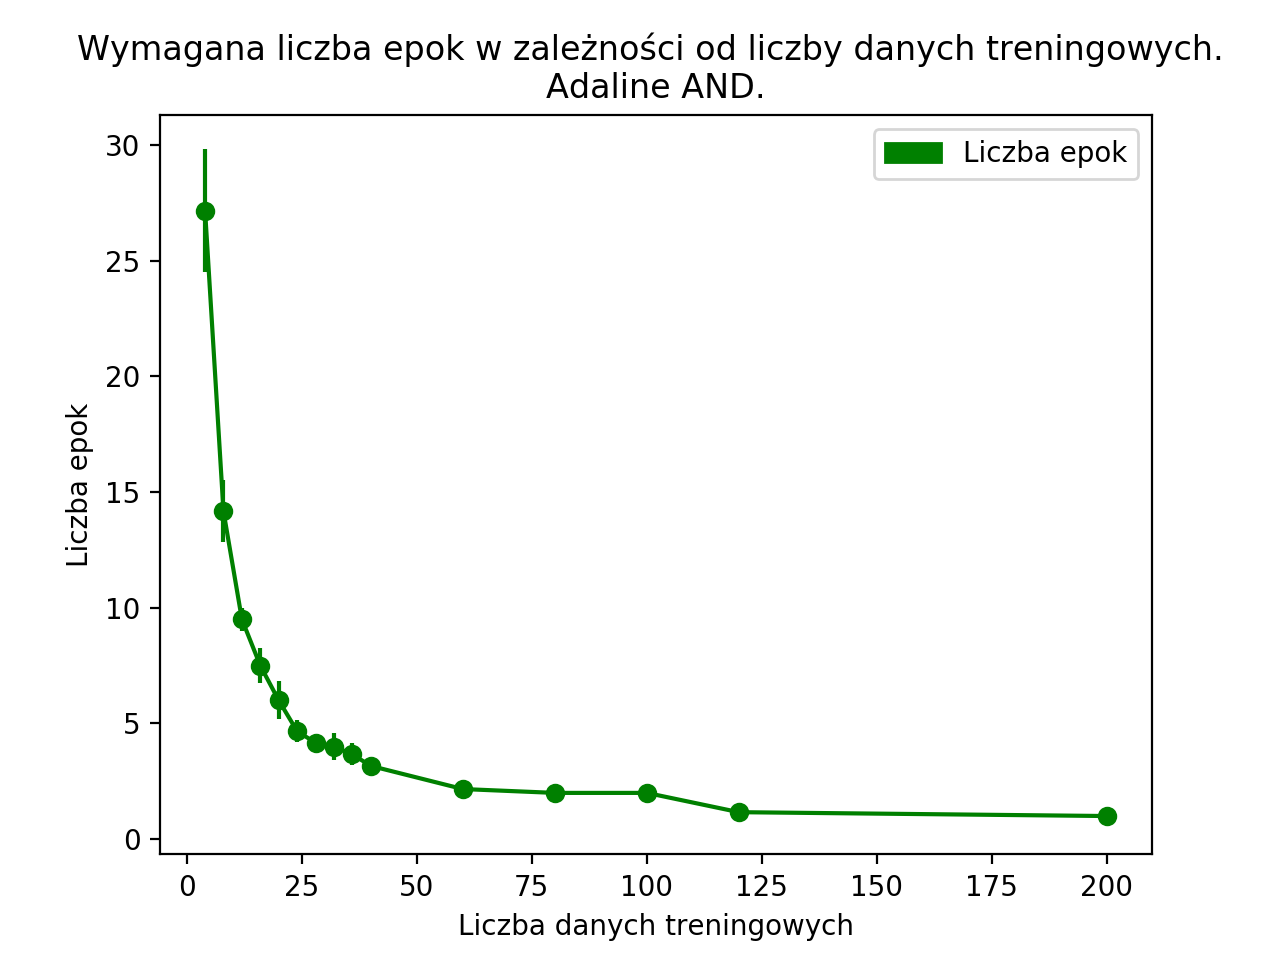
\includegraphics[width=0.5\textwidth]{epoki_dane_adaline_and.png}
		
	\end{figure}	 
	Na podstawie powyższego wykresu wyraźnie widać, że wraz ze wzrostem liczebności zbioru treningowego maleje liczba epok wymaganych do wyuczenia Adaline. Dzieje się tak dlatego, że podczas jednej epoki dostosowujemy wagi więcej razy.\\[0.5cm] 
	
	Wymagana liczba epok do wyuczenia Adaline w zależności od stałej uczenia na wykresie 2 poniżej:
	
	\begin{figure}[h]

		\centering
		\caption{}
		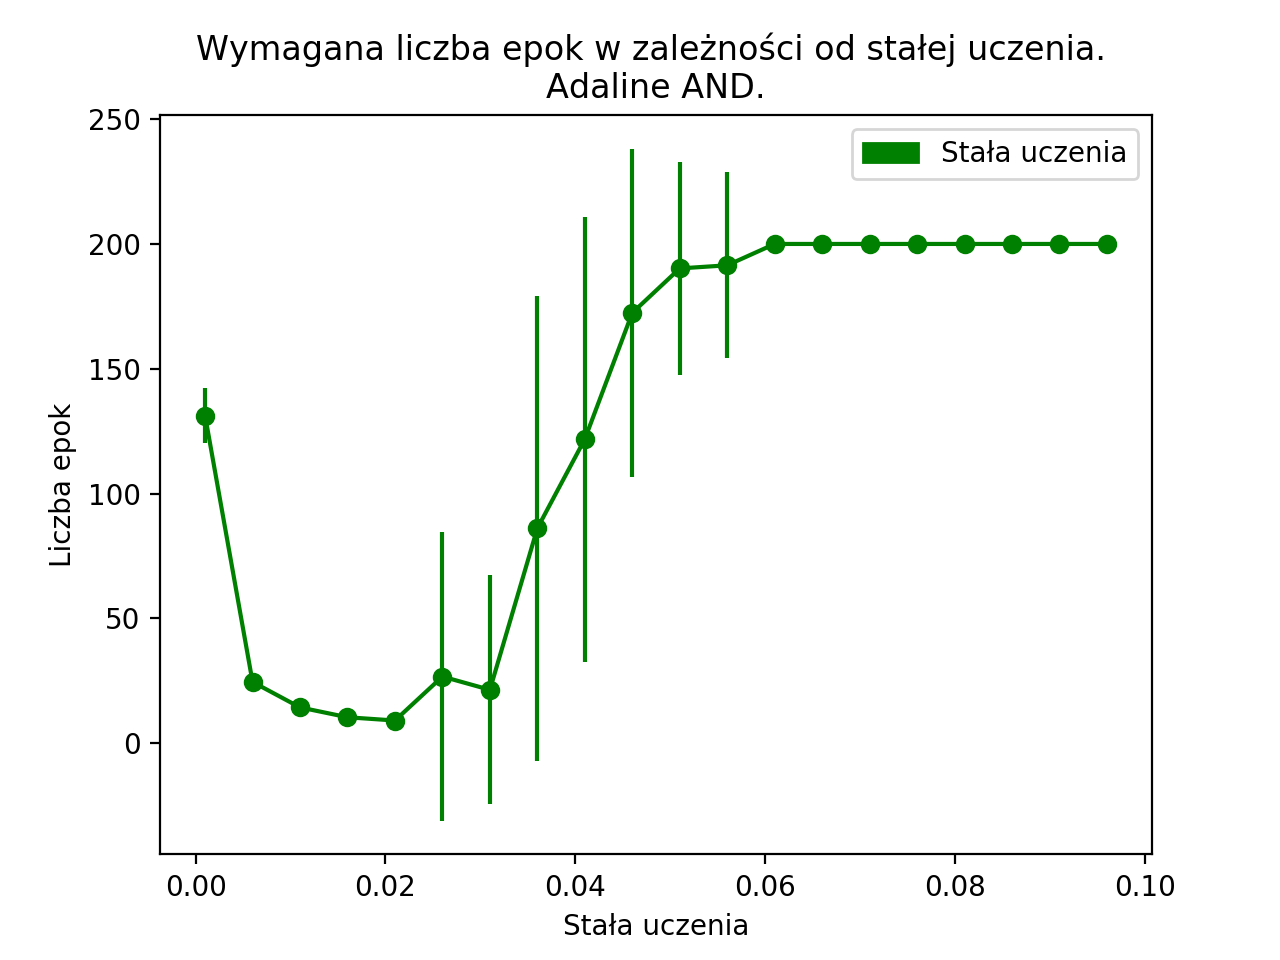
\includegraphics[width=0.5\textwidth]{epoki_rate_adaline.png}
		
	\end{figure}   
	Na podstawie powyższego wykresu wyraźnie widać, że zależność liczby epok od kroku uczenia ma pewne minimum. Istnieje taki zakres wartości stałej uczenia w której Adaline wyucza się najszybciej. Oznacza to, że wartość kroku uczenia nie może być ani zbyt mała ani zbyt duża.
	\newpage
	Wymagana liczba epok do wyuczenia Adaline w zależności od zakresu initializowanych wag na wykresie 3 poniżej:
	
	\begin{figure}[h]

		\centering
		\caption{}
		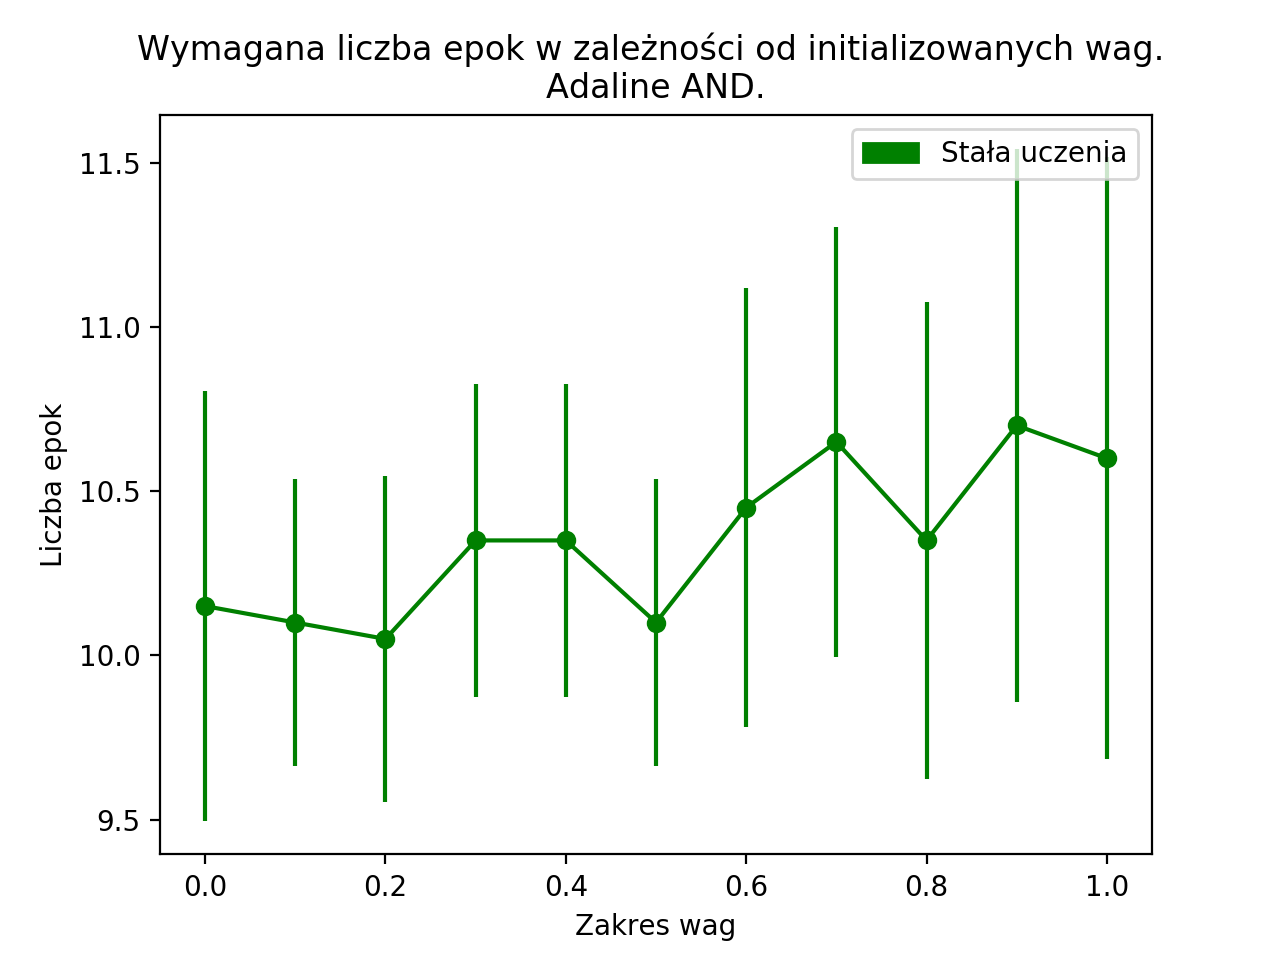
\includegraphics[width=0.5\textwidth]{epoki_wagi_adaline_and.png}
		
	\end{figure}   
	Zakres wag początkowych nie ma większego znaczenia w tym przypadku. Każdy z zakresów charakteryzuje się dużą wariancją i brakuje stabilnych wyników.
\newpage
	\subsection{Perceptron}
	\subsubsection{Funkcja aktywacji unipolarna}
	Wymagana liczba epok do wyuczenia perceptronu prostego dla funkcji aktywacji unipolarnej w zależności od wielkości zbioru uczącego na wykresie 4 poniżej:
	\begin{figure}[h]
		\centering
		\caption{}
		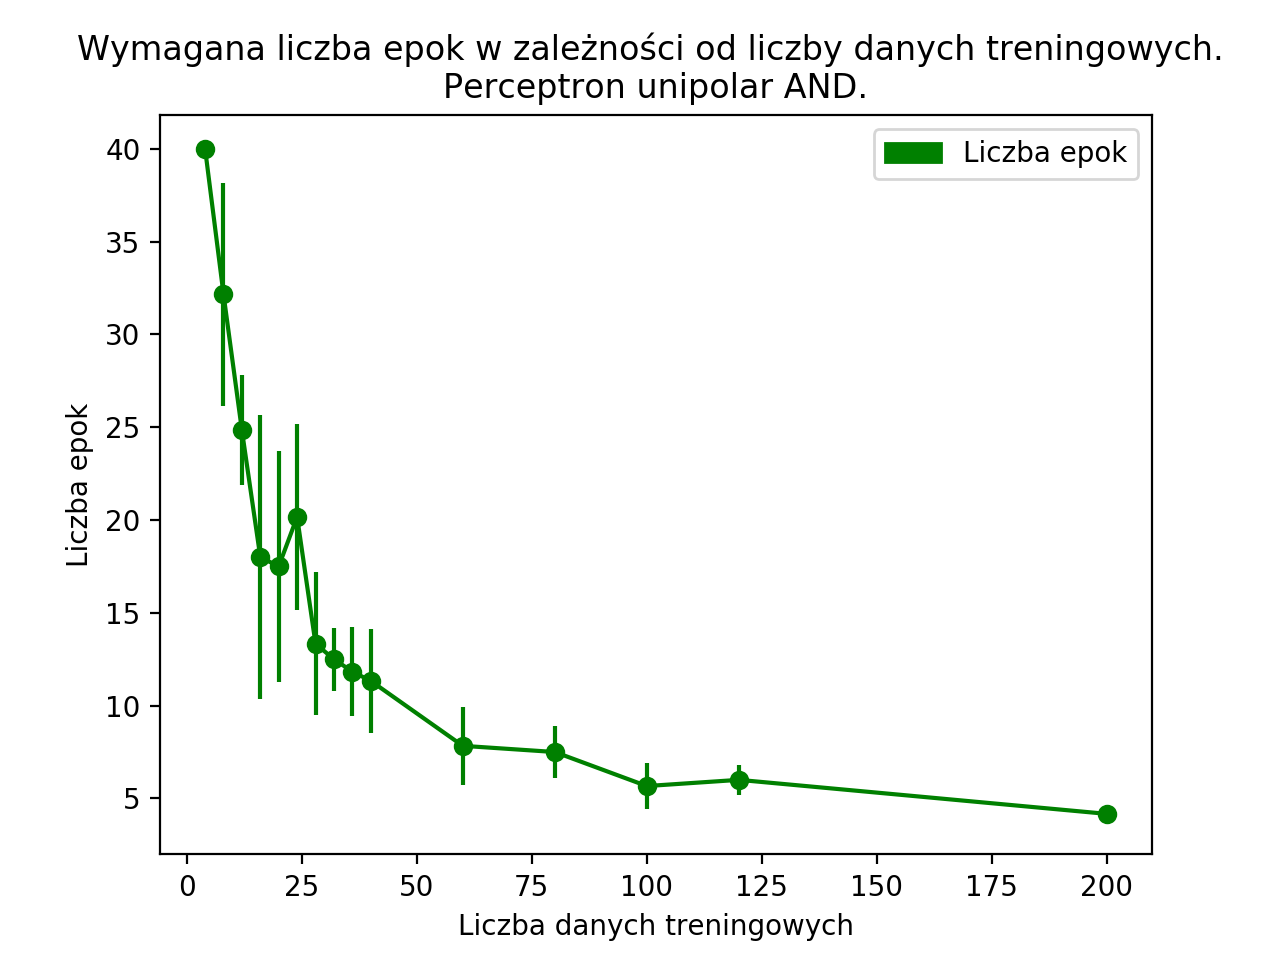
\includegraphics[width=0.5\textwidth]{epoki_dane_perceptron_unipolar_and.png}
	\end{figure}
	
	Wnioski do tego wykresu są analogiczne do wykresu 1. Jak w przypadku Adaline.\\[0.5cm]
	
	Wymagana liczba epok do wyuczenia perceptronu prostego dla funkcji aktywacji unipolarnej w zależności od wielkości zbioru uczącego na wykresie 5 poniżej:
	
	\begin{figure}[h]
		\centering
		\caption{}
		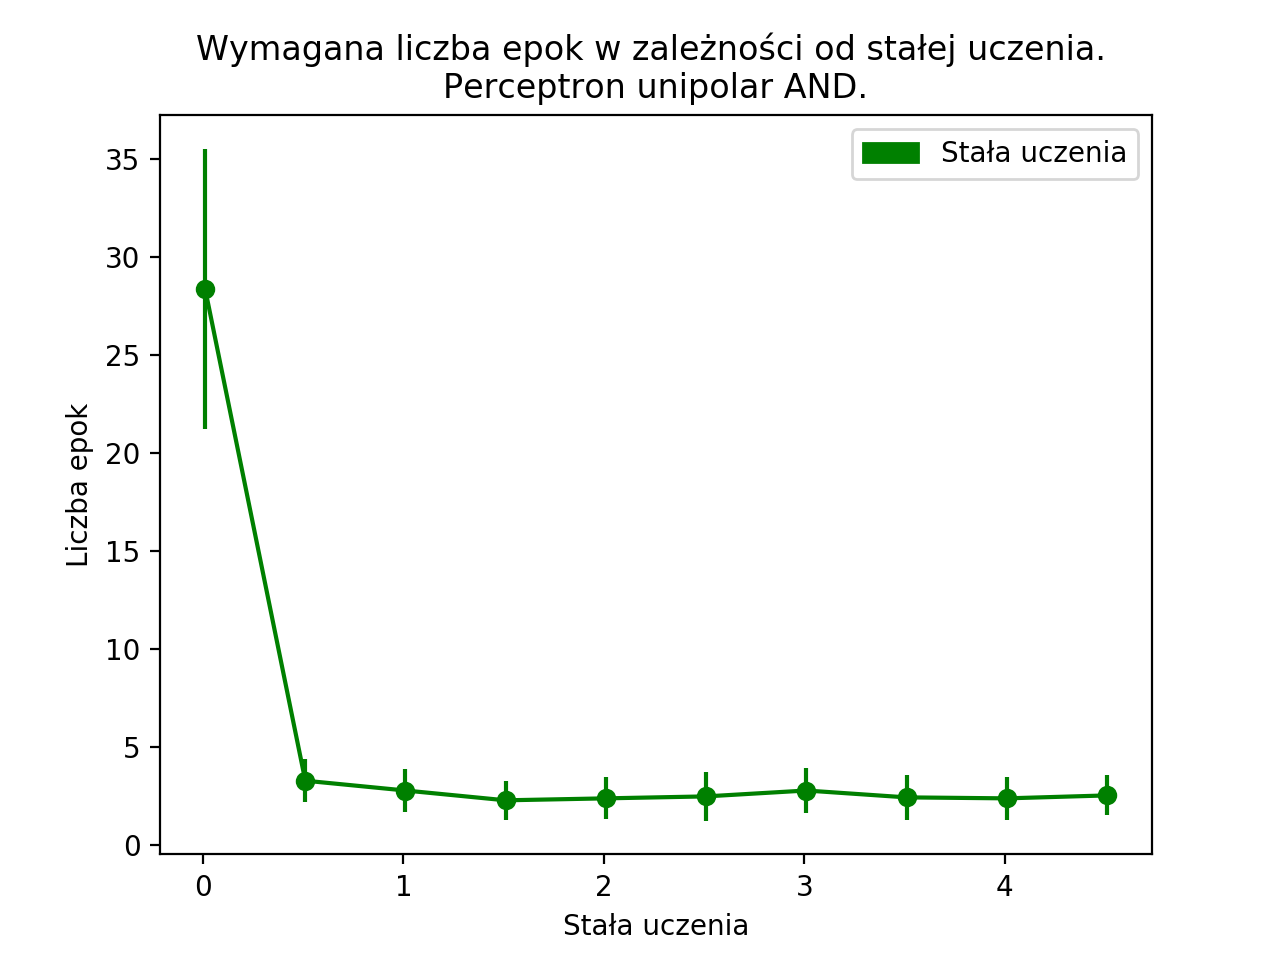
\includegraphics[width=0.5\textwidth]{epoki_rate_perceptron_unipolar.png}
	\end{figure}
	
	Uczenie perceptronu nie ma nic wspólnego z algorymem gradientu prostego. Nie ma więc znaczenia jak duża będzie stała uczenia. Wagi będą po prostu przeskalowane.
	\newpage
		Wymagana liczba epok do wyuczenia perceptronu prostego dla funkcji aktywacji unipolarnej w zależności od wielkości zbioru uczącego na wykresie 6 poniżej:
	
	\begin{figure}[h]
		\centering
		\caption{}
		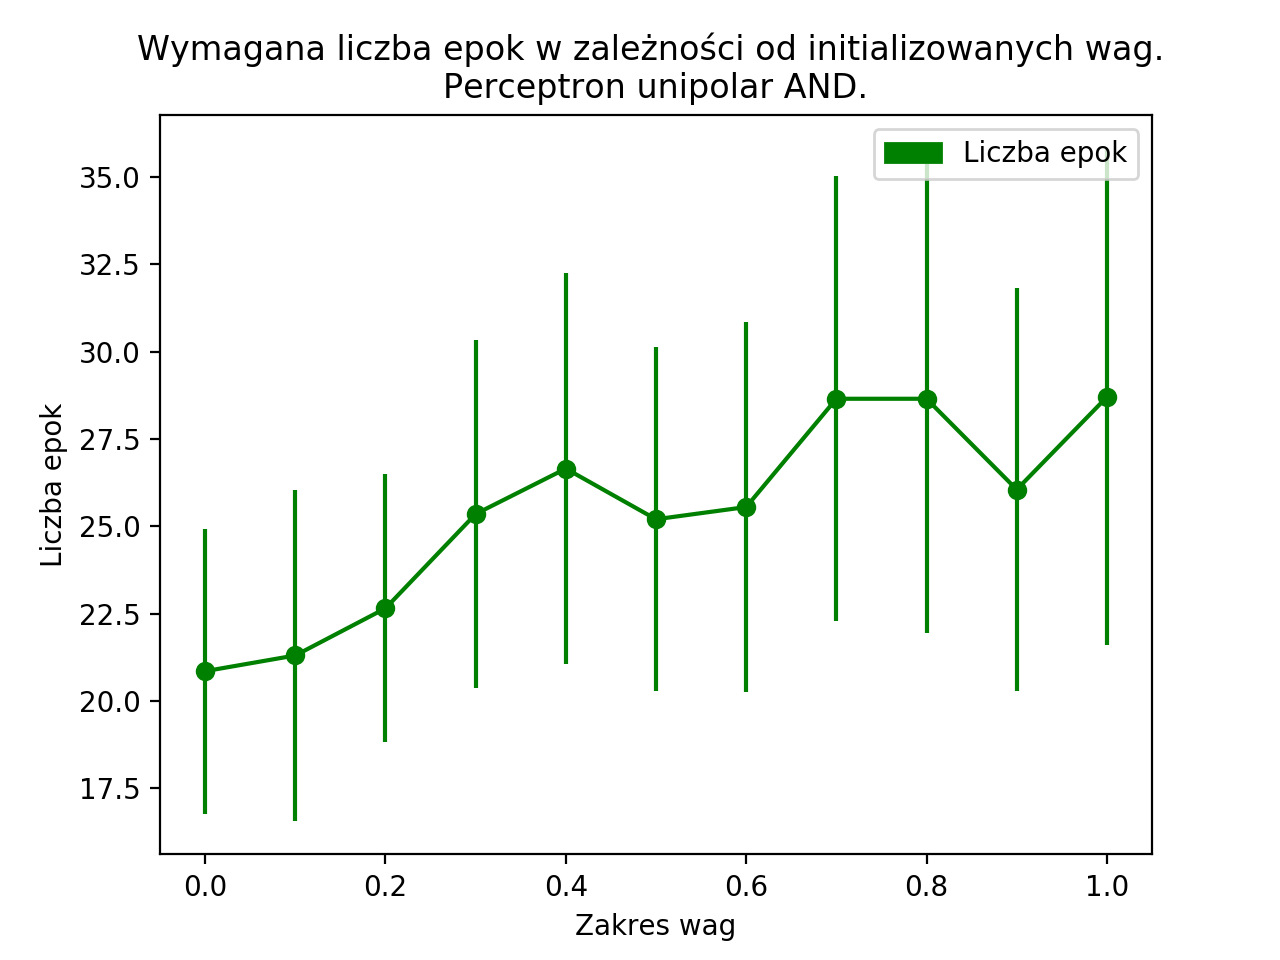
\includegraphics[width=0.5\textwidth]{epoki_wagi_perceptron_unipolar.png}
	\end{figure}
	
	Wyniki są obarczone dużą wiariancją. Dla bardzo małego zbioru treningwego można wywnioskować pewien trend rosnący, jednakże przy większym zbiorze treningowym, zakres initializowanych wag nie wpływa na szybkość uczenia.
	\newpage
	\subsubsection{Funkcja aktywacji bipolarna}
	Wymagana liczba epok do wyuczenia perceptronu prostego dla funkcji aktywacji bipolarnej w zależności od wielkości zbioru uczącego na wykresie 7 poniżej:
	\begin{figure}[h]
		\centering
		\caption{}
		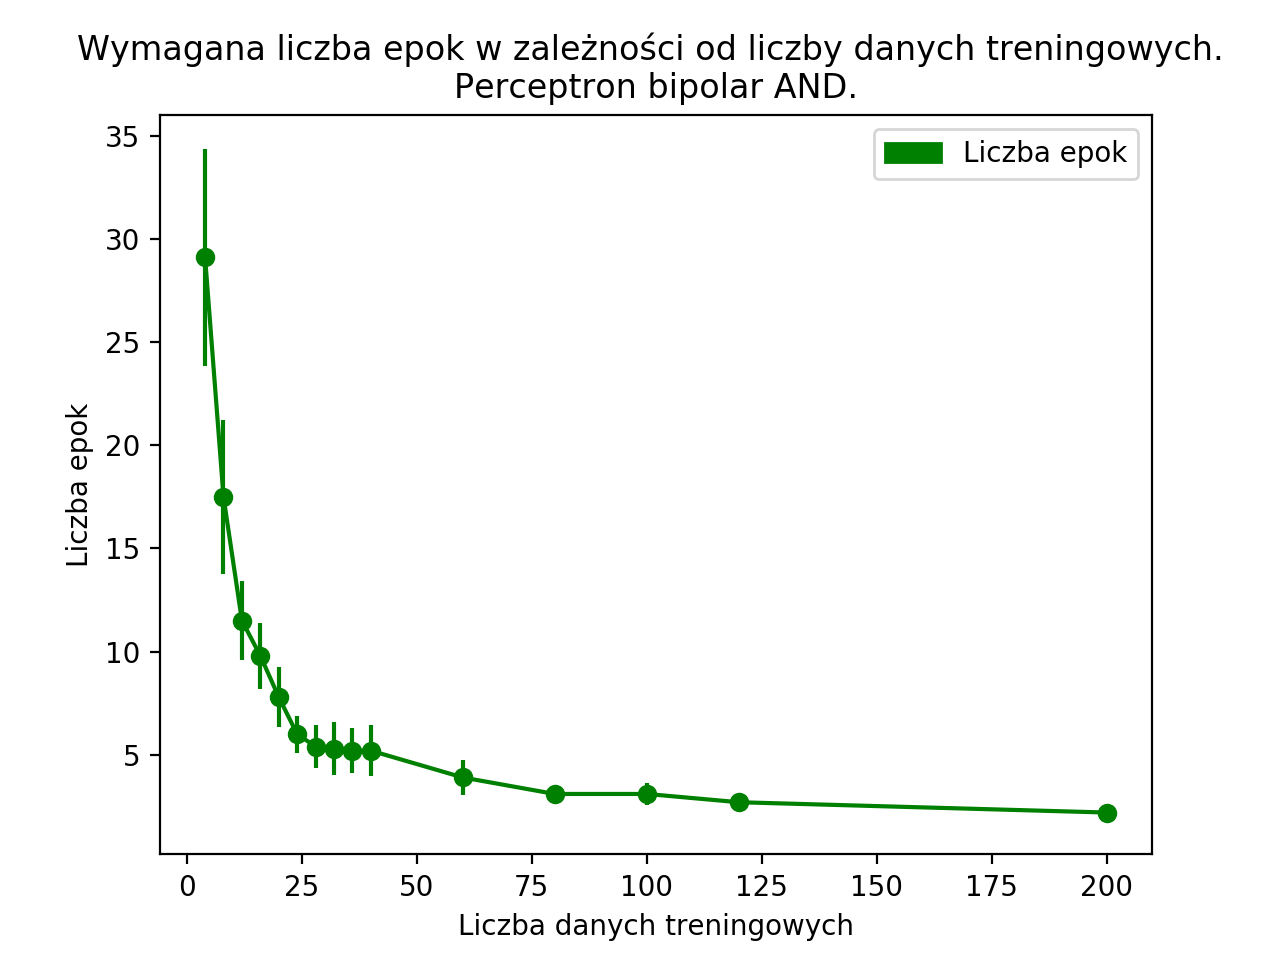
\includegraphics[width=0.5\textwidth]{epoki_date_perceptron_bipolar.png}
	\end{figure}

Wnioski do tego wykresu są analogiczne do wykresu 1. Jak w przypadku Adaline.\\[0.5cm]

	Wymagana liczba epok do wyuczenia Adaline w zależności od zakresu initializowanych wag na wykresie 8 poniżej:
	
	\begin{figure}[h]

		\centering
		\caption{}
		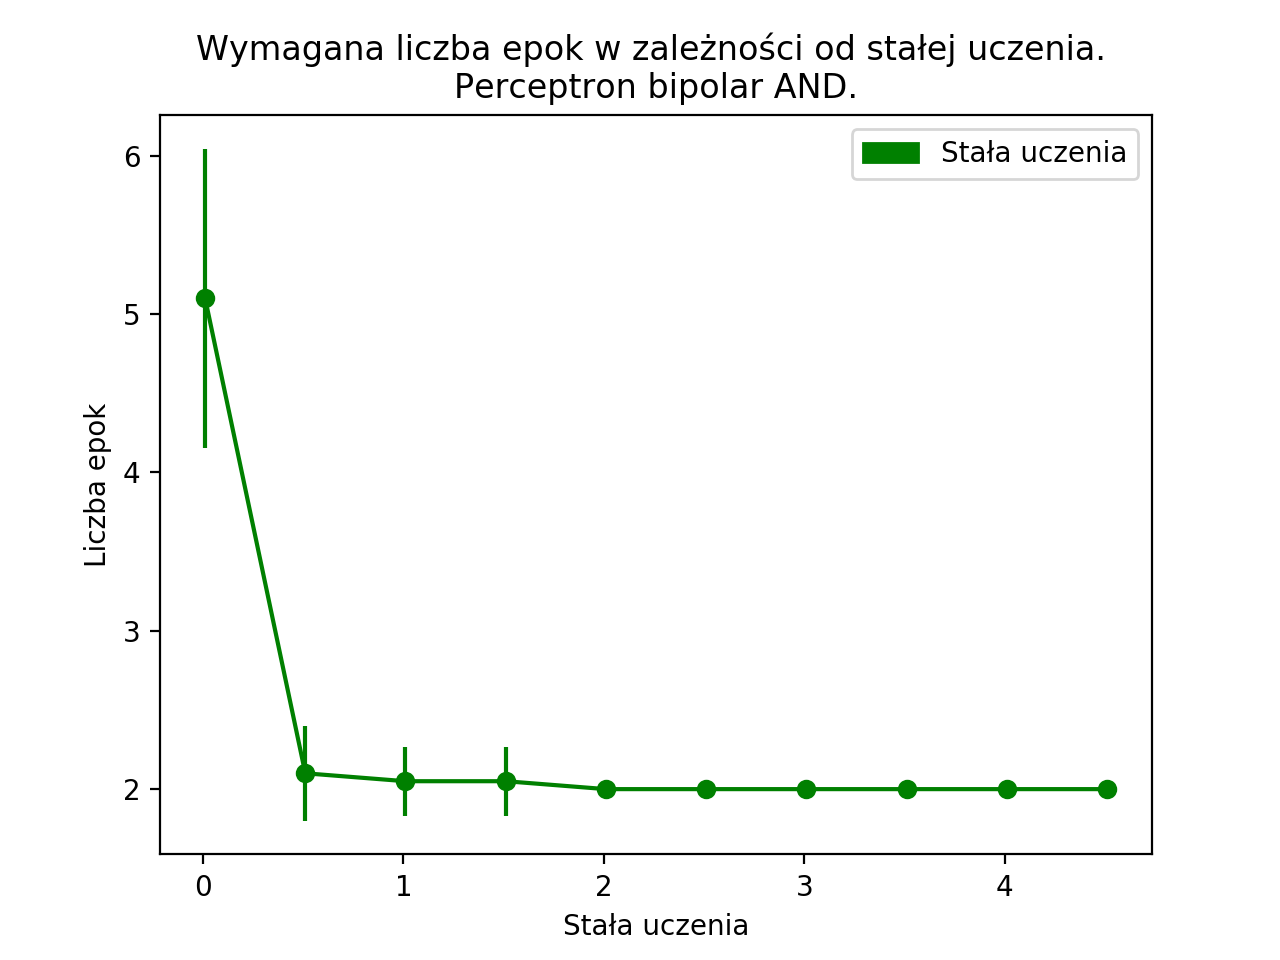
\includegraphics[width=0.5\textwidth]{epoki_rate_perceptron_bipolar.png}
		
	\end{figure}  
	Uczenie perceptronu nie ma nic wspólnego z algorymem gradientu prostego. Nie ma więc znaczenia jak duża będzie stała uczenia. Wagi będą po prostu przeskalowane.
		\newpage
	Wymagana liczba epok do wyuczenia Adaline w zależności od zakresu initializowanych wag na wykresie 9 poniżej:
	
	\begin{figure}[h]

		\centering
		\caption{}
		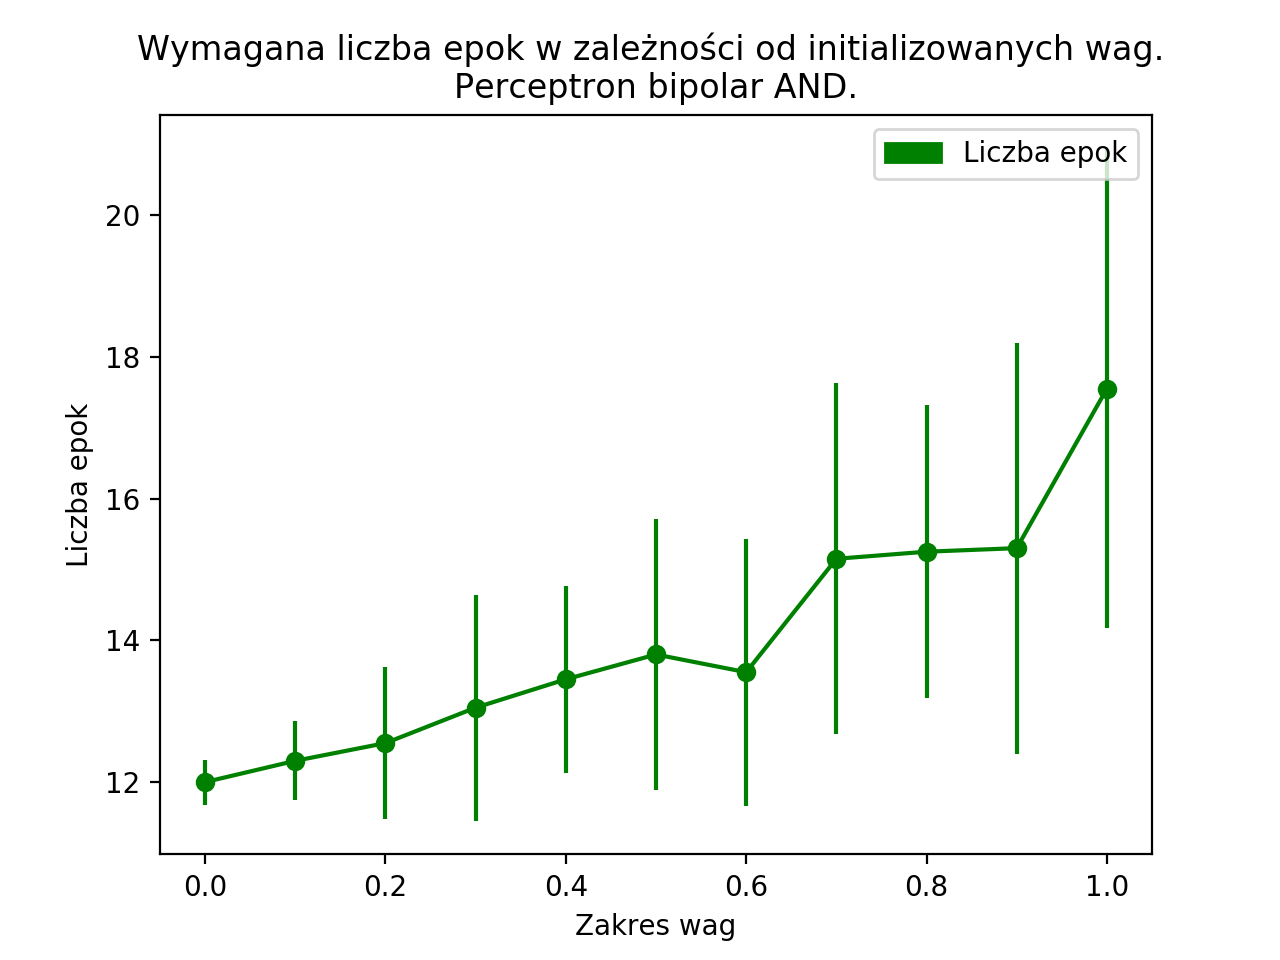
\includegraphics[width=0.5\textwidth]{epoki_wagi_perceptron_bipolar.png}
		
	\end{figure}   
	
	\subsection{Przykładowy wykres błędu w trakcie uczenia}
	Wykres błędu w zależności od epoki na wykresie 10 poniżej:
	
	\begin{figure}[h]
		\centering
		\caption{}
		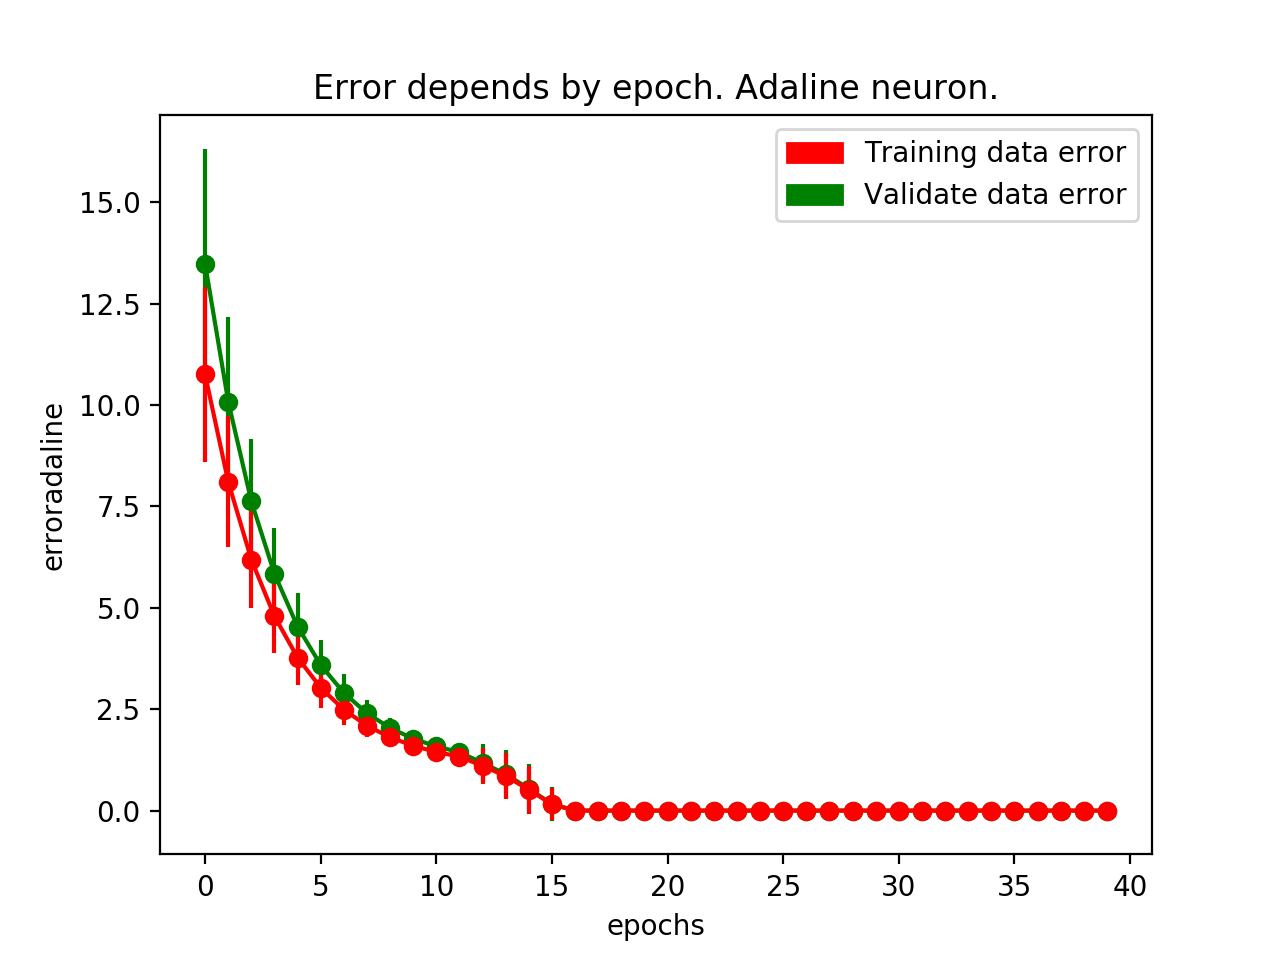
\includegraphics[width=0.5\textwidth]{adaline_and.png}
		
	\end{figure}  
\newpage	
	\section{Podsumowanie}
	
	
	Na podstawie przeprowadzonych badań w trakcie ćwiczenia zauważono, że w przypadku Adaline krok uczenia ma znaczenie w przeciwieństwie do perceptronu prostego. Dla Adaline wartość kroku uczenia nie może być ani zbyt mała ani zbyt duża. Gdy będzie zbyt mała będzie potrzeba zbyt wielu epok aby wyuczyć model, a w przypadku dużego kroku uczenia mamy do czynienia ze zjawiskiem eksplodującego gradientu. Dla perceptronu prostego stała uczenia nie może być zbyt mała z tego samego powodu, jednakże w przypadku jak będzie ona duża to nie wływa ona na jakość uczenia.\\[0.3cm]
	
Dla obydwóch modeli, liczba wymaganych epok maleje wraz z liczbą elementów w zbiorze treningowym.\\[0.3cm]
	
Dla obydwóch modeli zakres wartości wag początkowych nie miał większego znaczenia w szybkości uczenia. Jedynie w przypadku bardzo małego zbioru treningowego, można zauważyć pewien trend. Dla bardzo małego zbioru treningowego, potrzebnych jest mniej epok gdy wagi są zbliżone do zera. \\[0.3cm]

Obydwa modele nie radzą sobie z problemami nieseparawoalnymi liniowo.\\[0.3cm]


\end{document}

